\documentclass{article}

\usepackage{graphicx}    % for handling figures in the document

\usepackage{amsmath}   % for math environments
\usepackage{amssymb}   % for special math symbols

\usepackage{booktabs}    % for making tables pretty
\usepackage{caption}

\usepackage{array}
\newcolumntype{K}[1]{>{\raggedright\let\newline\\\arraybackslash\hspace{0pt}}m{#1}}    %for having a single variable width column

\usepackage{tabularx}    % for handling tables with variable width columns and text wrapping
\usepackage{tabulary}     % for handling tables with variable width columns and text wrapping

\usepackage{color, soul}    % for highlighting

\usepackage[round,
				    authoryear,
				    colon]{natbib}    %for the bibliography
\bibliographystyle{plainnat}

\usepackage{url}    %for handling of urls in bibtex file
\def\UrlBreaks{\do\/\do-}    %use to break urls at hyphens

\usepackage{pdflscape}    % for landscape orientation of pages

\usepackage[margin=1in]{geometry}    % to get 1-inch margins

\title{Chapter 2:\\Incorporating Roadway-Level Variables in Bicycle Demand Models}
\author{Timothy Brathwaite}
\date{}

\begin{document}
\maketitle

\section*{\abstractname{}}
In this chapter, I describe a new approach for incorporating roadway-level variables into bicycle demand models. The approach is based on a novel concept called the ``zone of likely travel'' and on the combination of decision trees from computer science with traditional discrete choice models. Both of these facets of the new approach will be described in detail. Beyond descriptions, this chapter includes an empirical application of the proposed techniques. The application demonstrates the feasibility and the utility of the new approach, showing in-sample and out-of-sample model improvements as well as policy-relevant levels of sensitivity to roadway-level variables. Finally, I present theoretical comparisons between the new approach and existing methods for using roadway-level variables in bicycle demand models. The approaches that are compared include analyses based on geographic buffers, bicycle environment factors, and combined bicycle route and mode choice models. The proposed approach is shown to inherit major benefits of these previous methods while avoiding many of their drawbacks.

\section{Introduction}
As noted in Chapter 1, agencies at every level of the United States (U.S.) government have begun to prioritize encouraging bicycle use. However, despite good intentions, these agencies still operate in a funding constrained environment. As such, agencies try to garner the greatest total benefit, subject to their budget constraints, by judiciously choosing projects to increase bicycling. One important class of projects is the installation of on-street bicycle infrastructure such as bicycle lanes, ``cycle tracks'' (i.e. protected bicycle lanes), bicycle boulevards, and ``protected intersections.'' In this context, agencies may want to get the greatest increase in bicycle usage out of a given budget for installing new on-street infrastructure.

Now, to determine the optimal bundle of installations (e.g. set of bike lanes), one needs to know how much a particular installation bundle will raise the bicycle mode share. This means that one requires a travel demand model with at least two features. First, `bicycle' must be explicitly modeled as an available alternative for at least some members of one's dataset. A travel demand model with this trait will henceforth be called a ``bicycle demand model.'' Secondly, one's model must be differentially sensitive to on-street infrastructure installations on different streets. This will allow agencies to meaningfully compare one set of proposed on-street infrastructure installations against another and select the installation bundles that will lead to the greatest increase in bicycle usage.

Although the two aforementioned requirements can be quickly conceived, few travel demand models meet these criteria. Amongst those travel demand models that do include bicycling as an explicitly modeled alternative, few models incorporate roadway-level variables such as bicycle lanes, traffic speeds, traffic volumes, and roadway slopes. The exclusion of such variables that are clearly relevant for the choice of bicycling leads to not only biased and inconsistent parameter estimates, but it leads to a lack of policy relevance for decision-makers that need to choose amongst projects that affect these roadway-level variables. Finally, amongst the precious few bicycle demand models that do incorporate these roadway-level variables, there remain striking theoretical drawbacks in the way that these variables are incorporated.

This chapter is a response to the aforementioned omissions and challenges of incorporating roadway-level variables into bicycle demand models. In the upcoming sections, I make the following contributions to the travel demand modeling literature. First, I present a novel methodology for incorporating roadway-level variables such as bicycle infrastructure into travel mode choice models. To do so, I (1) develop a new representation for the spatial environment between a person's origin and destination, and (2) I draw upon algorithmic methods (decision trees) that complement the traditional, linear-in-parameters travel demand model. The proposed techniques offer the potential for improved model accuracy compared to current modeling approaches based on geographic buffers around one's origin and/or destination or ``pedestrian/bicycle environment factors.'' Relative to route choice models, the new procedure has two advantages. It is far less computationally demanding than a route choice model, and the new procedure avoids the theoretical drawbacks of applying a route choice model estimated solely on cyclists to a mixed population of cyclists and non-cyclists. Secondly, I present an empirical application and policy forecast using the proposed method. In doing so, I demonstrate the feasibility of the new approach and the benefits of accounting for roadway-level variables rather than omitting them.

The rest of the chapter is organized as follows. First, I review the current approaches for incorporating roadway-level variables into mode choice models in Section \ref{sec:lit_review}. This review is largely the same as in Chapter 1, except for an additional discussion of how this chapter's methodology addresses the issues with previous approaches. Secondly, I present the details and theoretical benefits of the proposed methodology in Section \ref{sec:methodology}. Third, I present an empirical application of the new techniques in Section \ref{sec:application} where I analyze the commute mode choices of residents in the San Francisco Bay Area\footnote{Because this chapter is oriented towards practice as opposed to research, the empirical comparisons are against a travel demand model without roadway-level variables. A comprehensive, quantitative comparison with the existing approaches for using roadway-level variables in bicycle demand models is left for future research.}. I estimate the proposed model, and I use it to forecast the effects of a planned, Bay Area bicycle infrastructure investment. Finally, Section \ref{sec:conclusion} concludes.

\section{Literature Review}
\label{sec:lit_review}
The current state of most mode choice models is that they focus on socio-demographic attributes of the decision makers and ``level-of-service" variables such as travel times (e.g. in-vehicle travel time, waiting time, access time, egress time), travel cost, and travel distances of various modes \citep{singleton_pedestrians_2013}. As noted above, mode choice models often omit variables that describe individual roadway segments and are of particular interest to policy makers and individual travelers: variables such as the presence of bicycle lanes or the speed limit on particular roadways. Such an exclusion affects transportation engineering in two major ways. First, the usefulness of current mode choice models for addressing policy questions, such as whether one proposed bicycle infrastructure plan will have a greater effect on bicycle demand than another possible plan, is greatly reduced when the relevant variables being altered do not even appear in one's model. Secondly, the ability of current models to accurately represent the choice processes of individuals may be reduced by omitted variable bias and the spatial autocorrelations that may occur due to the omission of these roadway-level variables \citep{goetzke_are_2003}. As noted in the introduction, this omission indicates a clear need for methods of integrating roadway segment information into mode choice models.

Thus far, roadway-level variables have been incorporated into mode choice models in three main ways: through the use of buffer-based (as in geographic buffers around a point in space) methods, through the use of pedestrian/bicycle environment factors, and through the use of route choice models \citep{guo_effect_2007, replogle_integrating_1995, nassir_choice_2014}. Each of these methods has their drawbacks. First, buffer-based methods require the arbitrary setting of a distance to use as the buffer length around the origin and/or destination. Secondly, it is not necessarily clear that all of the area around a person's origin and/or destination is important to a traveler's mode choice decision, especially since an individual will be traveling in a particular direction and only the attributes of the built environment in that direction are expected to be relevant. Thirdly, if multiple spatial attributes are to be included in one's mode choice model, it is not clear whether or how those multiple variables should be combined for entry into the model. 

Arbitrariness or the ad-hoc nature of methods for combining multiple attributes that one considers important is also a criticism of pedestrian/bicycle environment factors \citep{ewing_travel_2001}. Such environment factors are often hand-crafted indices that are thought to measure the ``quality" of the built environment for walking and bicycling \citep{replogle_integrating_1995}, but the coefficients used to combine different variables into a single score are typically chosen through ``expert-judgement" as opposed to being chosen through a systematic method. Systematic methods of combination (such as using principle components analysis or factor analysis) exist, but the results of using such techniques are often considered difficult to interpret. 

In contrast to the buffer-based and bicycle environment factor methods, an approach that may seem promising is to combine bicycle route-choice models and mode choice models. This approach uses a bicycle route-choice model to measure the quality of various routes, and then uses the log-sum of the route-choice model to measure the overall quality of the bicycling option. The log-sum measure is then used as the explanatory variable for the bicycling alternative within a mode choice model. This approach avoids the pitfalls of using (1) ad-hoc or difficult-to-interpret methods to quantify the quality of bicycling for an individual or (2) of considering irrelevant geographies as with buffer based methods. 

However, there are at least three problems with the use of combined route and mode choice models. First, transportation datasets that are used for mode choice models are typically travel diaries, and such datasets do not typically collect information on the precise routes that individuals, particularly cyclists, use. Since these datasets cannot be used to construct route choice models, the coefficients from route choice models developed on one set of individuals are then used to represent the sensitivities of different individuals in the mode choice dataset. Secondly, route choice models are often only estimated on those for whom one has observed route choices--i.e. on current cyclists. The sensitivities of current cyclists are then taken to be the same as the sensitivities of non-cyclists, and this is probably an inaccurate assumption. Nevertheless, the log-sum measure based on cyclists' sensitivities are used to represent the overall quality of bicycling for non-cyclists. Lastly, it typically takes a long time to estimate and forecast with route choice models \citep{nassir_choice_2014}. This is because both the initial estimation and the forecasting procedures of route choice models used in practice depend on lengthy route generation processes that limit the practical usefulness of such models.

\subsection{Summary}
\label{sec:lit_review_summary}
To summarize, there are currently three major techniques for  incorporating roadway-level variables into mode choice models: buffer-based methods, ``pedestrian/bicycle environment factors,'' and route-choice models. Each of these three methods has their drawbacks. The main issues with these methods are as follows.
\begin{enumerate}
\item Buffer-based methods include streets that are likely to have low impact one's decision of whether or not to cycle, and they simultaneously exclude streets that are likely to be influential in one's decision making process.

\item Bicycle environment factors lack a systematic and easily-interpreted method for combining the various variables of importance into a single measure of the quality of one's environment for bicycling.

\item Route choice models are based solely on the decisions of one non-representative sub-population---cyclists, and then they are applied to a completely different sub-population (i.e. non-cyclists), even though the preferences of these sub-populations may greatly differ.

\item The choice set generation processes commonly used in route choice models lead to long computation times, thereby reducing the immediate usefulness of such models for practitioners.
\end{enumerate}

In the next section, I will detail the proposed methodology for including previously omitted roadway-level variables into mode choice models and addressing the four issues listed above.


\section{Methodology}
\label{sec:methodology}

The proposed methodology for making mode choice models sensitive to roadway-level variables is comprised of three main parts. 

First, I create a novel representation of the built-environment between one's origin and destination called the ``zone of likely travel." The new representation aims to better capture relevant roadways and areas than traditional buffer-based methods. Conceptually, instead of forming buffers around a person's origin and/or destination, the zone of likely travel can be conceived of as a buffer around the shortest path between an individual's origin and destination.

Secondly, I propose the use of decision-trees as a supervised dimensionality-reduction technique. After building the decision tree using the decision to commute by bicycle or not as the dependent variable, the series of conjunctive statements that comprise its output are taken as discrete interactions that describe a person's cycling environment. Unlike ``objective'' bicycle environment-factors, these discrete interactions are easily interpreted combinations of the extracted roadway-level variables such as the percentage of roadways with various types of bicycle infrastructure on them and the deciles of roadway slopes in a person's zone of likely travel. Moreover, unlike subjective bicycle environment-factors, these variable combinations are systematically created and (by construction) highly predictive of whether a person chose to commute by bicycle. 

Thirdly, I propose the use of the hybrid decision-tree logit model, as described by \citet{steinberg_hybrid_1998}, to integrate the variable combinations that describe the environment that a person travels through with traditional mode choice models. In this step, one merely places the set of discrete interactions into the bicycle utility of one's mode choice model as dummy variables and conducts one's usual model estimation procedure.

In the three subsections that follow, Sections \ref{sec:zone_of_likely_travel} - \ref{sec:hybrid_tree_logit_models}, I provide motivation, intuition, and implementation details for each of the three steps in the methodology.

\subsection{Zone of Likely Travel}
\label{sec:zone_of_likely_travel}
In attempting to alleviate the issues of omitted roadway-level variables described in the introduction, there were essentially two options. First, I could have taken an approach that was similar in spirit to current buffer-based and bicycle environment factor methods. These methods directly operate at spatial levels of aggregation that are based on areas as opposed to being based on precise travel routes. Alternatively, I could have taken an approach that is similar to that of route choice models. In doing so, one would judge the quality of specific routes that an individual could use to travel from his/her origin to his/her destination and then aggregate those judgements in some way to describe the quality of the environment between one's origin and destination. Given the aforementioned data, generalization, and computational issues of route choice models, I decided to sidestep those problems and use an approach similar to buffer-based and bicycle environment factor methods. The first step in such a procedure was to determine the spatial area(s) for each person that would be used to judge the quality of that person's bicycling environment.

In particular, I introduced the concept of a ``zone of likely travel" as the spatial area to be used in or modeling efforts. The ``zone of likely travel" is a polygon between an person's origin and destination that aims to include the roadways that an individual is thought to be likely to travel on. Conceptually, it can be thought as a buffer around the straight line between an individual's origin and destination. The main motivation for such zones was twofold. First, I wished to avoid using buffers around an individual's origin and destination because they may be composed of many roadways that are irrelevant to a person's decision of whether to travel by bicycle. For example, these could be roadways that are near one's origin but travel in the opposite direction from one's destination and vice versa. Secondly, I wanted to be sure that the characteristics of roadways between a person's origin and destination were captured, especially since the area between a person's origin and destination can be much larger than the area around the person's origin and destination. The zone of likely travel achieved both of these goals.

To actually construct the zones of likely travel, I relied on a revealed preference study by Dill and Gliebe (\citeyear{dill_understanding_2008}) that describes the percent difference between the length of observed and shortest paths of cyclists, based on the length of the cyclist's shortest path in one mile increments. Their findings regarding these percent differences are shown in Figure \ref{fig:dev_dist}. The basic idea is that once one knows the length of the shortest path from an individual's origin to destination, one can draw a buffer around that path such that the buffer contains the routes that the cyclist may take if they deviate from the shortest path. With the results of Dill and Gliebe (\citeyear{dill_understanding_2008}), I used the following series of steps to create each person's zone of likely travel:
\begin{enumerate}
\item  Calculate the length of the shortest path between the individual's origin and destination

\item Based on the data in Dill and Gliebe (\citeyear{dill_understanding_2008}), find the mean percent difference in length between observed and shortest paths for trips whose shortest paths are in the same mileage category as the current individual's trip

\item Using the mean percent difference in length, calculate the expected bicycle trip length for the current individual's trip.

\item On a map, draw a straight line between the individual's origin and destination.
\label{alg:straight_line_step}

\item Calculate an ``offset distance" by subtracting the length of the straight line from the expected bicycle trip length and then dividing by two.

\item At an ``offset distance" away, in both directions orthogonal to the straight line drawn in step \ref{alg:straight_line_step}, draw parallel straight lines. See the green and purple lines in Figure \ref{fig:init_zone}.

\item Draw a box by connecting the start and end points of the three straight lines. See Figure \ref{fig:init_zone}.

\item Associate each corner of the box, as well as the origin and destination, with their closest roadway intersections.
\label{alg:intersection_association_step}

\item Starting at the roadway intersection nearest the origin and moving in a single consistent direction, clockwise or counter-clockwise, create a polygon by the determining the shortest path on the actual road network between the current roadway intersection and the next roadway intersection from step \ref{alg:intersection_association_step}.
\end{enumerate}
Note that Figure \ref{fig:init_zone} illustrates an intermediate stage in the construction of the zone of likely travel, and Figure \ref{fig:actual_zone} depicts an example of an actual person's zone of likely travel. Once the zones of likely travel are constructed for each person, one can begin collecting variables and combining them to describe the quality of an individual's bicycling environment. This process will be described in the following subsection.


\begin{figure}
\centering
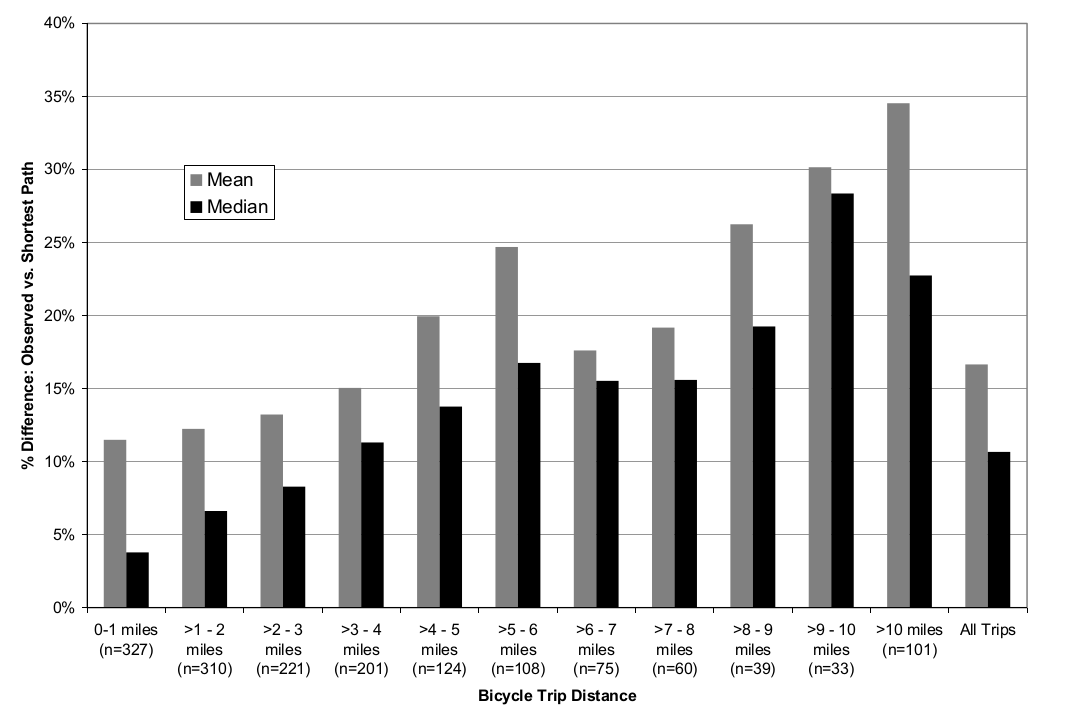
\includegraphics[width=\textwidth]{../images/deviation_distribution}
\caption{Percent difference between observed and shortest paths by bicycle trip length \citep{dill_understanding_2008}}
\label{fig:dev_dist}
\end{figure}

\begin{figure}
\centering
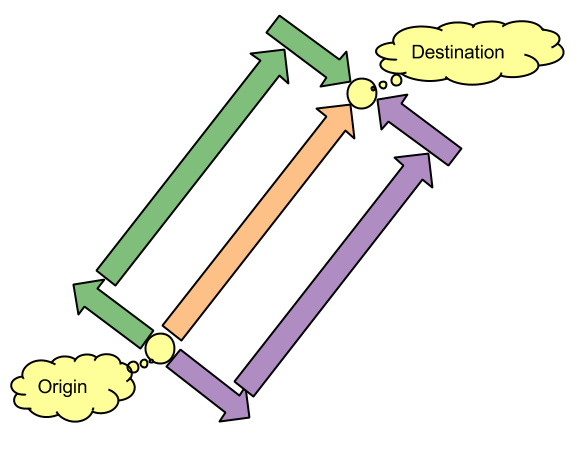
\includegraphics[width=\textwidth]{../images/zone_of_likely_travel_initiation}
\caption{Initialization of the Zone of Likely Travel}
\label{fig:init_zone}

\centering
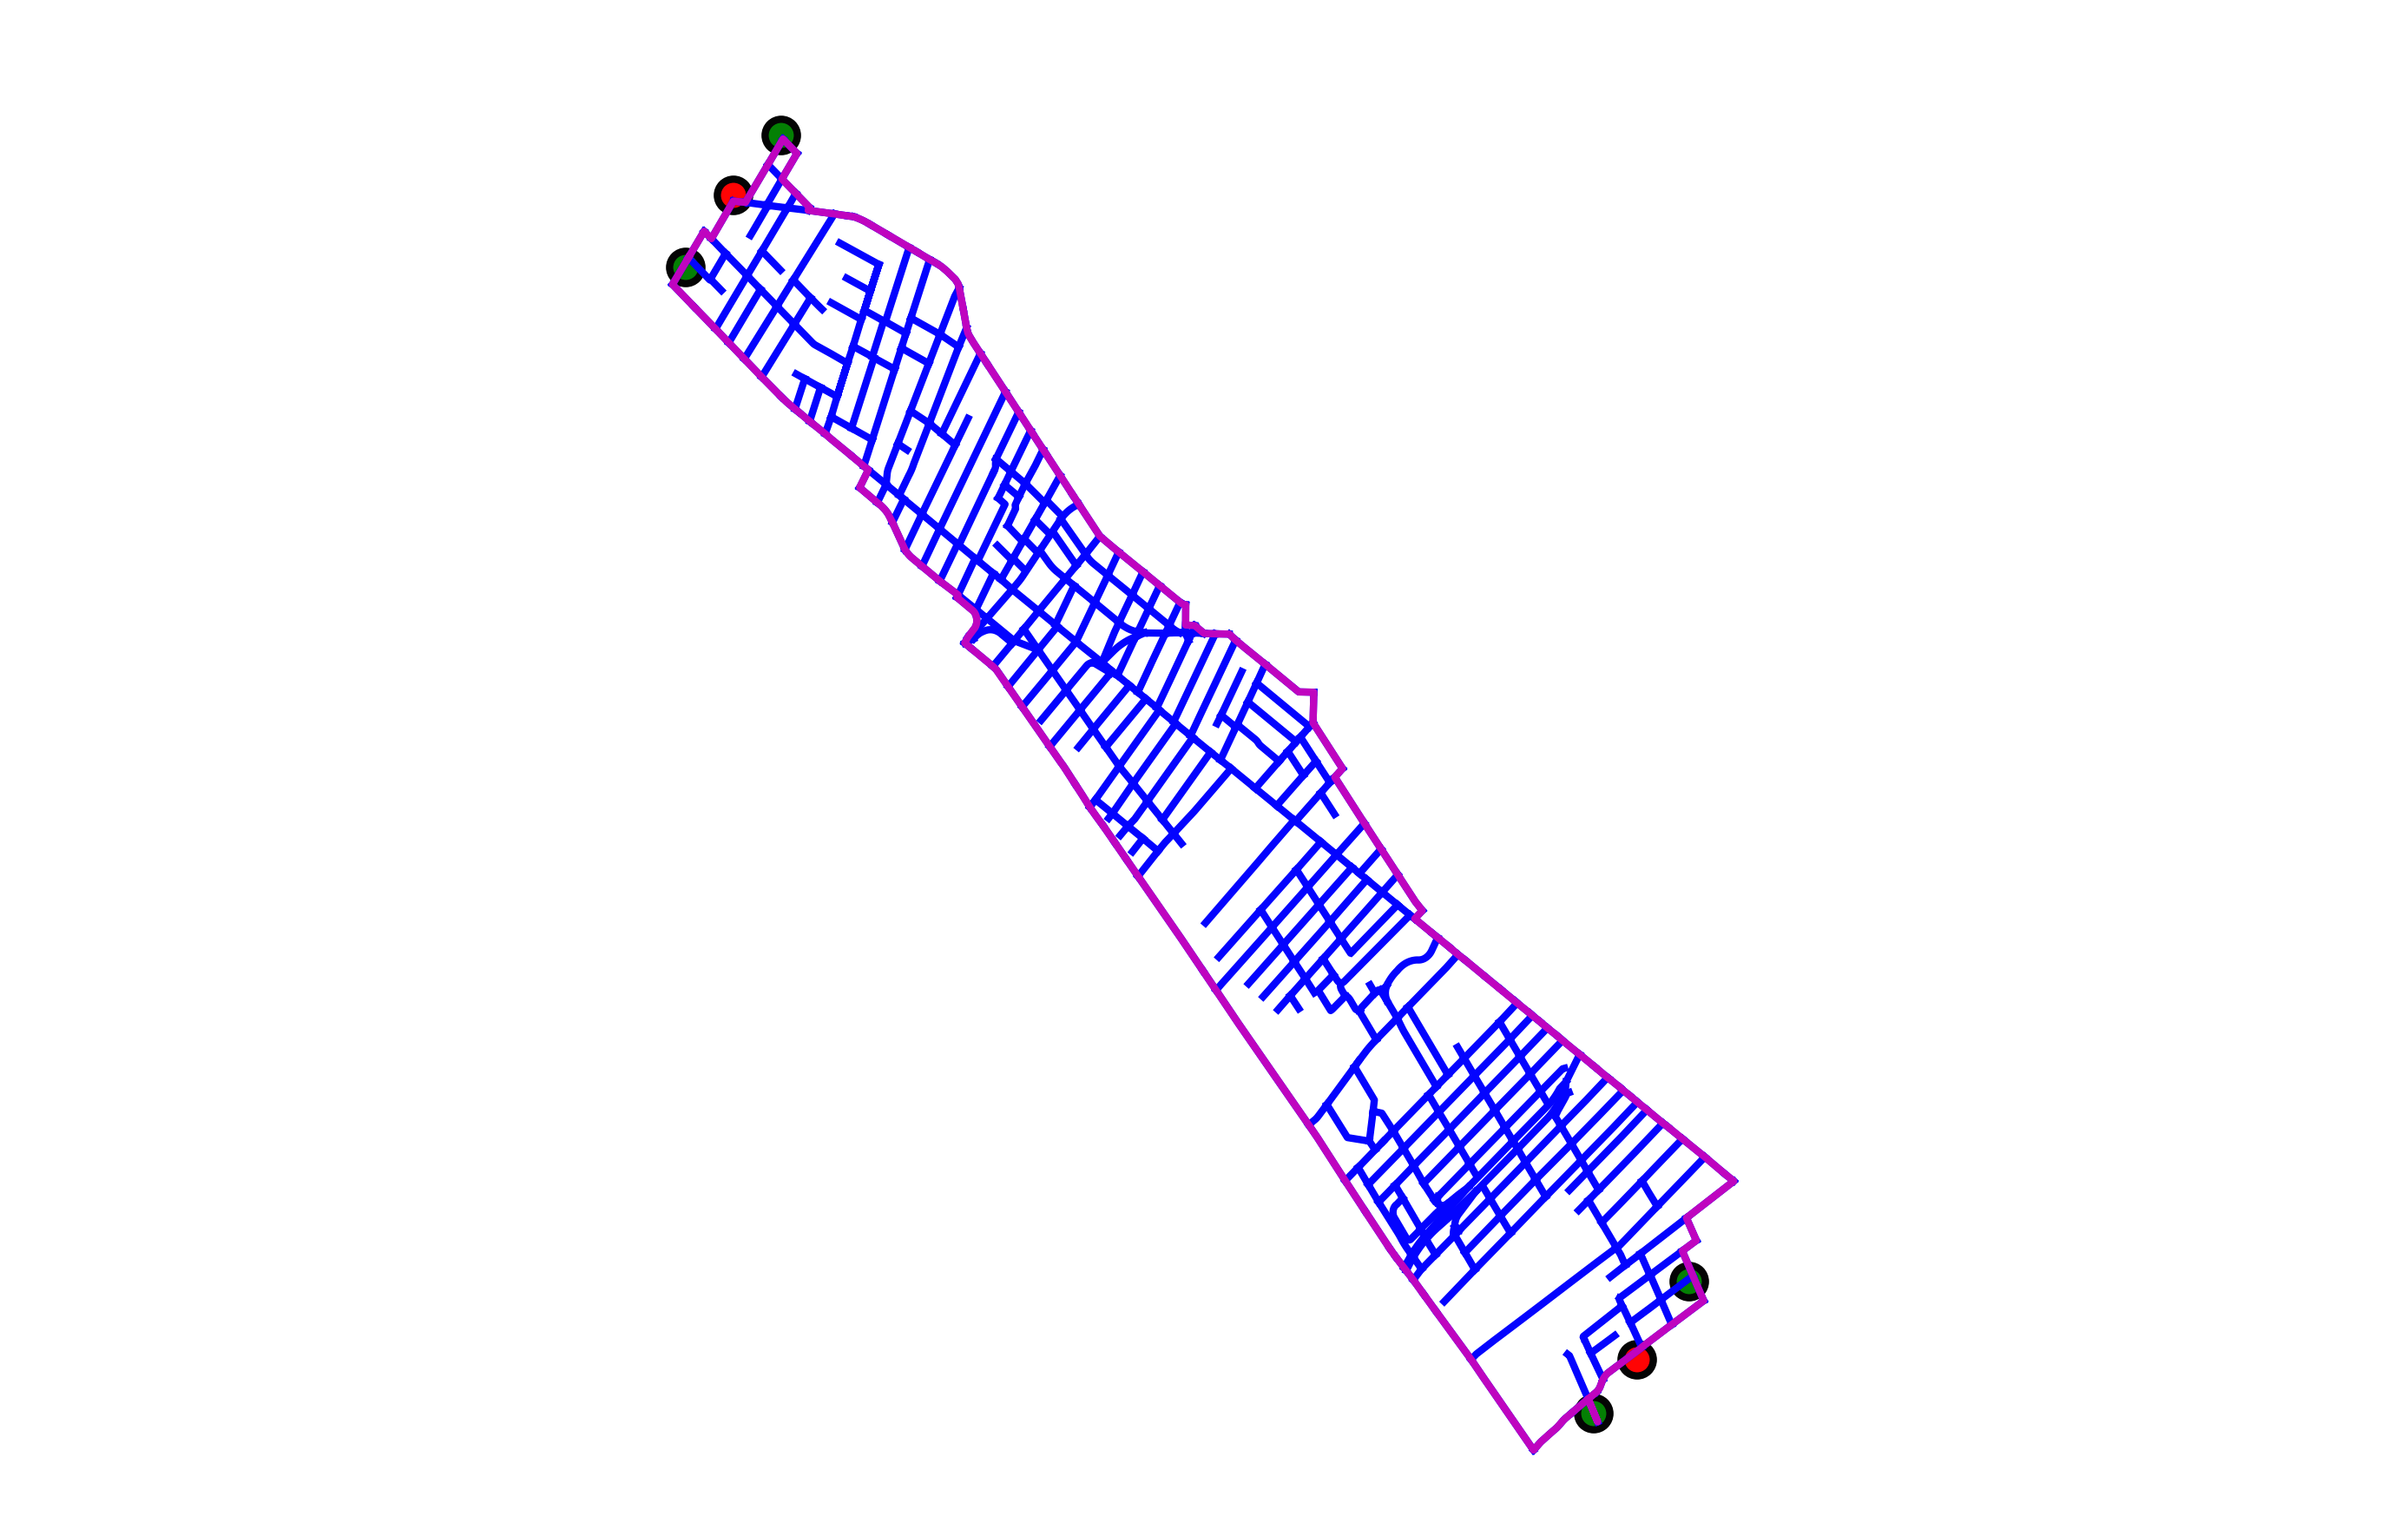
\includegraphics[width=\textwidth]{../images/zone_example}
\caption{Example of an actual Zone of Likely Travel}
\label{fig:actual_zone}
\end{figure}


\subsection{Decision Trees for Dimensionality Reduction}
\label{sec:trees_for_dimension_reduction}
Given a constructed zone of likely travel, the next step in the methodology is to collect and combine roadway-level variables from the zone in order to describe its bicycling environment. In general, the variables collected from each zone will be determined by the needs, resources, and interest of each researcher. However, the basic idea of this part the methodology is to collect as many variables describing the bicycling environment as one can. 

To determine the variables one collects, one might choose to be creative with one's variable definitions. For instance, one might measure the percentage of miles along the shortest path from one's origin to destination that have speed limits below a certain speed. This would be an indicator of perceived traffic safety along one's most direct travel route. One might also choose to describe the distribution within the zone of each variable of interest as finely as possible. As a concrete example, consider the following. One is often curious about the effects of the following categories of roadway-level variables on the probability that a person chooses to commute by bicycle: types of bicycle lanes, designated bicycle routes, and off-street paths; traffic speeds; traffic volumes; roadway slopes.

The approach that I took in this study was to describe the entire distribution of these variables instead of merely using point  estimates. For example, instead of merely using the mean of all the roadway slopes within the zone, I instead measured the deciles of the empirical distribution of roadway slopes in the zone.

Once one has collected all of the variables that one is interested in, one might have a large corpus of highly correlated variables. For example, I had more than thirty measured variables. As such, directly entering all of these variables into one's mode choice model is not expected to be effective\footnote{Note, this point is corroborated by the results in Table 1 of Chapter 4. There, point estimates of the variables of interest are directly entered into the bicycle utility equation, and still, only the variable for bicycle lanes is statistically significant. Contrast those results to the results shown in Table \ref{table:combined_results} of this chapter where 7 of the 8 dummy variables representing the output nodes of the tree were statistically significant.}. Instead, the variables are combined in a way that reduces the dimensionality of the terms that are added to the mode choice model. Moreover, I wanted the variable combinations to be objective, interpretable, and predictive of whether or not a person choose to commute by bicycle. Because of these requirements, I avoided standard dimensionality reduction techniques such as principle component analysis and factor analysis.These methods have been characterized as difficult to interpret, and the resulting variable combinations are not necessarily predictive of a particular dependent variable. Similarly, I avoided the use of bicycle-environment factors since such factors are constructed subjectively using expert opinions.

The approach I settled on was using a decision tree to perform the variable combination, where the dependent variable was whether or not a person chose to commute by bicycle. Provided that the tree that one constructs is of low depth, the tree and its resultant variable combinations will be easily interpretable. Each output node will be able to read as series of conjunctive statements such as ``this node represents observations whose zones of likely travel meet condition 1 and condition 2 and not condition 3," etc. Additionally, because decision trees are constructed with the express purpose of accurately classifying observations, the variable combinations that are created as the decision tree's output nodes will be precisely those that are highly predictive of whether one chooses to commute by bicycle or not. For an in depth discussion of decision trees and strategies for their construction, see Chapter 4.


\subsection{Hybrid Decision Tree-Logit Models}
\label{sec:hybrid_tree_logit_models}
The final step in the methodology is to construct the hybrid decision tree-logit model. As described by \citet{steinberg_hybrid_1998}, this model takes the output nodes of the decision tree and adds them as ``dummy variables'' to the systematic utility of one's discrete choice model. Given that the decision tree is estimated specifically to predict the choice of bicycling or not, I added the dummy variables to the specification of the systematic utility of bicycling as opposed to the utility of any of the other modes.

Now, the main motivation for placing the output nodes of the decision tree into the bicycle utility of one's discrete choice model is to create a link between the effect of the roadway-level variables and the probability that a person bicycles. However, there are other benefits that come from using this technique. First, discrete choice models and decision trees are generally complementary techniques \citep{steinberg_hybrid_1998}. Decision trees work by finding relationships between the dependent variable and local partitions of the space of explanatory variables. In contrast, discrete choice models are typically used to estimate relationships (i.e. the $\beta$'s) that hold globally, for all observations, regardless of one's location in the space of explanatory variables. Given that both techniques have been used to predict discrete outcomes with much success, one may hope to do even better by combining the two techniques. Secondly, the decision tree has (in our case) solely been used to relate the roadway-level variables to the choice of bicycling. Conversely, discrete choice models in transportation usually only account for socio-demographics and level-of-service variables. Combining the two models and re-estimating the coefficients allows us to interpret the effects of roadway-level variable while controlling for socio-demographics and level-of-service and vice versa.

\section{Application}
\label{sec:application}
For an empirical application, I jointly modeled the commute mode choices of individuals in San Francisco, Berkeley, and Oakland. These cities were chosen because I had data on a sample of individual commute mode choices through the 2012-2013 California Household Travel Survey, and because it was feasible for me to acquire, clean, and standardize the needed geospatial data. In the following subsections, I describe the data used in the application, as well as the model specification that is used as my point of comparison. I then present the model results (both the decision tree and hybrid decision-tree logit model), and use the model to forecast the change in the number of bicycle riders that is expected to come from the Telegraph Avenue Complete Streets project in Oakland.

\subsection{Data}
As mentioned above, the primary dataset for this application is the 2012 California Household Travel Survey (CHTS). The CHTS was a one day travel diary taken from a stratified sample of households throughout the state of California and portions of Nevada. It was a stratified sample, one-day travel diary, and it collected detailed information on individual's activities, locations, sociodemographics, household structure, and travel modes. The complete data collection effort is described in \citep{california_department_of_transportation_2010-2012_2013}. From the complete data set, only individuals who both lived and worked or lived and attended school in either Oakland, Berkeley, or San Francisco were extracted and retained for model estimation. 

Beyond filtering based on geography and trip-purpose, I post-processed the raw CHTS data to construct the final dataset used for model estimation. In particular, I combined the data on individual trips into tours, defined a ``chosen travel mode'' for each tour, determined the available travel modes for each tour, and assembled the level-of-service variables for each tour. For this study, I used the level-of-service (travel costs, times, and distance) estimates provided by the San Francisco Metropolitan Transportation Commission (MTC). As a result, the set of possible alternatives in our example was defined to be the same as the categories used by MTC. Specifically, eight travel mode alternatives were specified. There were three driving modes, each differentiated by the number of passengers: drive-alone, shared-ride with two passengers, and shared-ride with three or more passengers. There were also three transit modes, each differentiated by their access and egress modes: walk-transit-walk (where walking is used for access and egress), drive-transit-walk, and walk-transit-drive. Finally, there were two non-motorized modes: walking and bicycling. For each tour, the travel mode that was used for the longest distance was used as the ``chosen travel mode'' for that tour. In total, the final data set included 1,015 tours, 87 of which had bicycling as the primary travel mode used on the tour.

Along with the CHTS data, I drew upon a suite of spatial data from each city and from MTC. Specific data types gathered include street shapefiles, bicycle infrastructure shapefiles, speed limits, topography, traffic analysis zones (TAZs), and city boundaries.

\subsection{Base Model}
The ``basic" model used for comparison in this chapter is based on MTC's current work-tour mode choice model \citep{san_francisco_metropolitan_transportation_commission_travel_2012}. It is essentially taken ``as-is" from MTC and is used as a point of comparison for this application. Minor alterations to MTC's model specification were made based on data availability and statistical considerations such as using removing insignificant variables. The largest difference between the MTC model and the model used in this chapter is that I use a multinomial logit model instead of a nested logit model. This decision was made in order to investigate the improvements that are possible in the simplest type of choice model used by MTC. The Maximum Likelihood Estimation (MLE) results of the basic model are presented in Table \ref{table:combined_results}, along wiith the results of the hybrid decision-tree logit model.

\begin{table}
\centering
\begin{tabular}{K{0.5\linewidth} rrrr}
\toprule
{} & \multicolumn{2}{c}{Standard Logit} & \multicolumn{2}{c}{Hybrid Tree-Logit} \\
Variables & \multicolumn{1}{c}{Parameter} & \multicolumn{1}{c}{$t$-Stat} & \multicolumn{1}{c}{Parameter} & \multicolumn{1}{c}{$t$-Stat} \tabularnewline
\midrule

ASC Shared Ride: 2 & -2.737 & -11.833** & -2.717 & -11.715** \\
ASC Shared Ride: 3+ & -2.852 & -12.228** & -2.831 & -12.110** \\
ASC Walk-Transit-Walk & -0.215 & -0.593\hphantom{*}\hphantom{*} & -0.167 & -0.462\hphantom{*}\hphantom{*} \\
ASC Drive-Transit-Walk & -3.414 & -7.332** & -3.370 & -7.237** \\
ASC Walk-Transit-Drive & -3.949 & -8.212** & -3.907 & -8.125** \\
ASC Walk & 1.421 & 5.281** & 1.404 & 5.228** \\
ASC Bike & -0.950 & -3.402** & -3.291 & -5.297** \\
Travel Time, units:min (All Auto Modes) & -0.112 & -7.912** & -0.112 & -7.887** \\
Travel Time, units:min (All Transit Modes) & -0.029 & -6.854** & -0.029 & -6.970** \\
Travel Cost, units:\$ (All Transit Modes) & -0.123 & -1.432\hphantom{*}\hphantom{*} & -0.124 & -1.442\hphantom{*}\hphantom{*}  \\
Travel Distance, units:mi (Walk) & -1.103 & -12.535** & -1.096 & -12.475** \\
Travel Distance, units:mi (Bike) & -0.345 & -7.470** & -0.219 & -4.066** \\
Household Size (Shared Ride 2 \& 3+) & 0.593 & 9.774** & 0.585 & 9.618** \\
Cross-Bay Tour (All Transit Modes) & 1.037 & 2.109*\hphantom{*} & 1.056 & 2.146*\hphantom{*} \\
Node 1 (Bike) & \_ & \_ & 1.402 & 2.816** \\
Node 2 (Bike) & \_ & \_ & 0.926 & 1.066\hphantom{*}\hphantom{*} \\
Node 3 (Bike) & \_ & \_ & 1.928 & 2.369*\hphantom{*}  \\
Node 4 (Bike) & \_ & \_ & 4.238 & 6.338** \\
Node 5 (Bike) & \_ & \_ & 2.370 & 3.798** \\
Node 6 (Bike) & \_ & \_ & 4.583 & 4.931** \\
Node 7 (Bike) & \_ & \_ & 2.612 & 3.585** \\
Node 8 (Bike) & \_ & \_ & 1.483 & 2.145*\hphantom{*}  \\

\multicolumn{5}{c}{}\tabularnewline
Log-likelihood & -1,409.071 & \multicolumn{1}{c}{} & -1,372.327 & \multicolumn{1}{c}{} \tabularnewline

\bottomrule
\multicolumn{5}{l}{Note: * means $\textrm{p-value} < 0.05$ and ** means $\textrm{p-value} < 0.01$.} \\
\multicolumn{5}{l}{\hphantom{Note: }\_ means the corresponding values do not apply to the given model.}\\
\end{tabular}
\caption{Base and Hybrid Decision-Tree Logit Model Results}
\label{table:combined_results}
\end{table}

\subsection{The Hybrid Decision Tree-Logit Model}
As shown by the log-likelihoods in Table \ref{table:combined_results}, the hybrid decision-tree logit model displays a greater in-sample fit to the data as compared to the base model. The greater fit is statistically significant as a log-likelihood ratio test of the hybrid decision-tree logit model versus the restricted base model has a p-value of approximately $1e^{-12}$.

Now, to interpret the results of the hybrid decision tree-logit model, one also needs the estimated decision tree. Figure \ref{fig:tree_results} shows the estimated tree, and Table \ref{table:var_descriptions} describes the names of the variables that appear in the estimated tree.\footnote{Note the variables used to construct the tree include: the percentage of roads having bike lanes on them, the percentage of roads having bike routes or ``share the road'' arrows (i.e. sharrows) on them, the deciles of roadway slopes within a zone, the total elevation change from one's origin to destination, the deciles of roadway speed limits, the length of the shortest path from one's origin to destination, the fraction of one's shortest path that has a speed limit of 20, 30, and 35 miles per hour or higher. Only a subset of these variables appear in the estimated tree shown in Figure \ref{fig:tree_results}.} A few interesting aspects of the hybrid decision tree-logit model are immediately apparent. First, the presence of bicycle lanes only affects those individuals in output nodes 3-5, where the shortest path between the individual's home and work is less than 3.01 miles. This underscores the importance of distance in determining whether an individual chooses to bicycle and whether the individual is strongly impacted by the installation of on-street bike lanes. Secondly, the numerous appearance of the slope variables highlights the importance of having a relatively flat bicycling environment\footnote{Note, basic node splitting procedures for tree construction are biased towards selecting variables (such as the ``slope\_xx'' variables) with many unique values \citep{kim_2001_classification}. However, I was not aware of this fact when conducting the study described in this chapter. Future research should investigate the sensitivity of the decision tree's interpretation to the use of unbiased splitting procedures.}. Finally, it is instructive that the variable at the top of the tree is the fraction of roadways along one's shortest path with roadways of 35 miles per hour or higher. This emphasizes the fact that individuals rarely commute by bicycle in regions where their most direct path is along roads with fast moving (i.e. unsafe) traffic.

\begin{figure}
\centering
    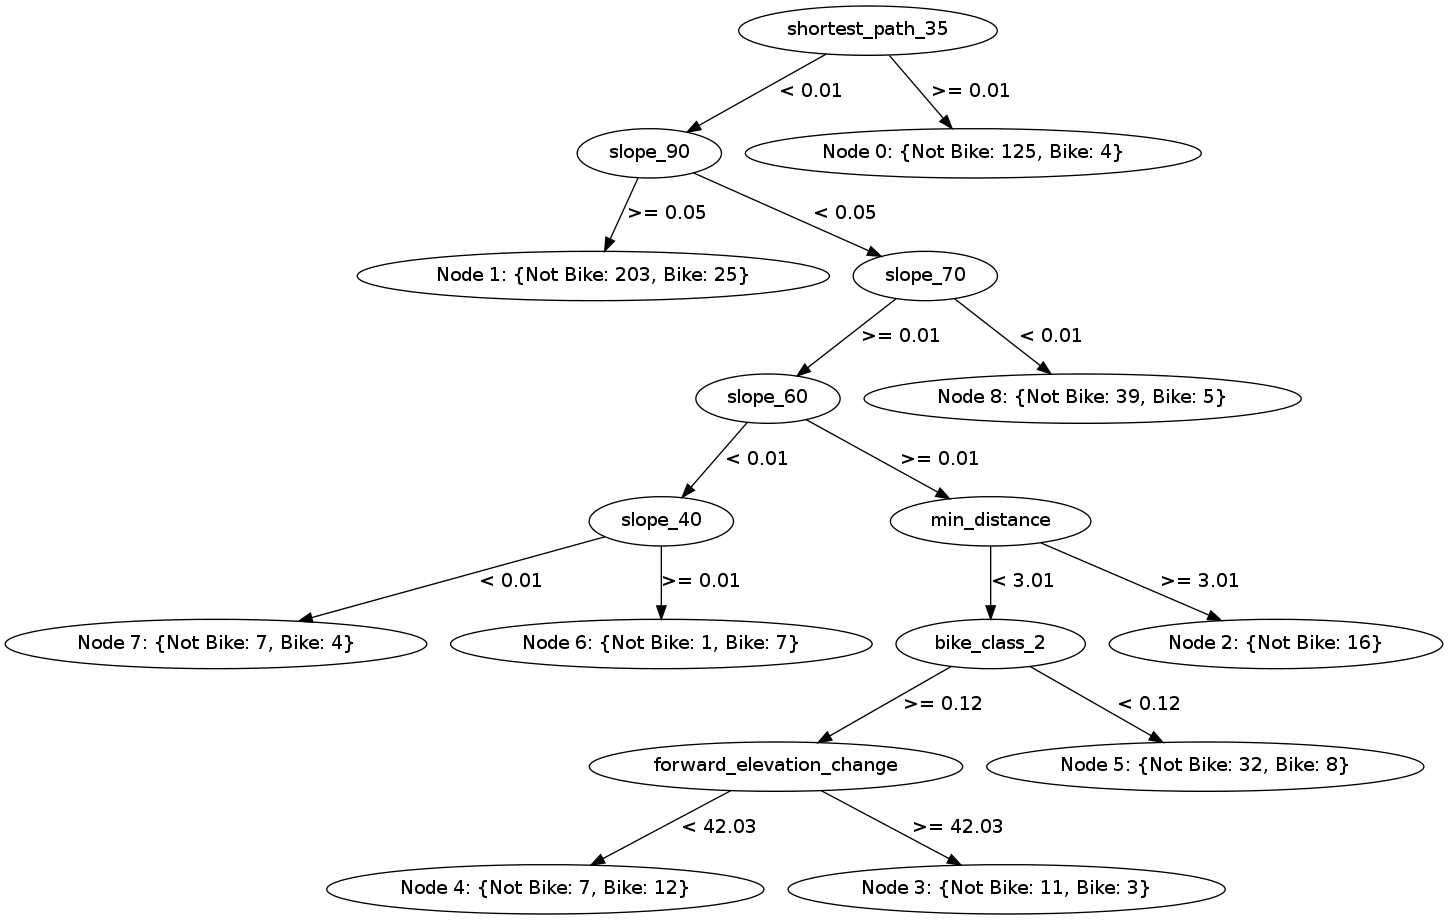
\includegraphics[width=\textwidth]{../images/test_graph_2}
    \caption{Estimation results for the decision tree}
    \label{fig:tree_results}
\end{figure}

\begin{table}
\begin{tabularx}{\textwidth}{l X}
\toprule
\multicolumn{1}{l}{Variable} & Descriptions \\
\midrule

shortest\_path\_35 & The ratio of miles of 35 mph roadways along the shortest path from one's origin to destination to the total roadway miles along the shortest path. 
 \\[1.2ex]
slope\_xx & The xx-percentile of the slopes in the zone of likely travel between one's origin and destination. 
\\[1.2ex]
min\_distance & The length, in miles, of the shortest path between one's origin and destination. 
 \\[1.2ex]
bike\_class\_2 & The ratio of roadway miles in one's zone of likely travel which have a bike lane on them to the total roadway miles in one's zone. 
\\ [1.2ex]
forward\_elevation\_change  & The absolute value of the change in elevation (in feet) between one's origin and destination. \\ 
\bottomrule

\end{tabularx}

\caption{Variable descriptions for variables in the classification tree}
\label{table:var_descriptions}
\end{table}

While the discussion so far has centered on the in-sample estimation results, I did assess the performance of the proposed methodology using out-of-sample testing. Specifically, I used two complementary metrics to assess the out of sample performance of the proposed method and the traditional logit model without roadway level variables: the out-of-sample log-likelihood and ``sensitivity.'' The log-likelihood measures the overall quality of a model's predicted probabilities. The sensitivity of a model measures the model's discriminative ability---it is the percentage of observations of a given outcome that are correctly classified\footnote{Note, for probabilistic models with multiple outcomes, an observation is classified as having the outcome with the highest predicted probability.} by one's model. Since this study is specifically focused on cycling, the models were judged with respect to their log-likelihoods overall and with respect to their sensitivity towards cycling.

To perform the out-of-sample testing, I used the ``0.632+'' bootstrap \citep{efron_1983_estimating, efron_1997_improvements}. Alternative techniques for performing the out-of-sample assessment were deemed inappropriate because of the dataset's small size (1,015 observations) and highly imbalanced nature (e.g. there were only 87 cyclists). For instance, a hold-out sample would have resulted in either few cyclists in the hold-out set or too few observations overall in the training set. Similarly, the small number of cyclists in each fold of cross-validation would have increased the variance of all the out-of-sample estimates. To sidestep these issues, I used 2,000 bootstrap samples of the data to re-estimate the models based on my proposed methodology and the traditional logit model. Each time, the log-likelihood and sensitivity were calculated for the observations that were not part of the bootstrap sample. The log-likelihood and sensitivity metrics were then averaged across the 2,000 bootstrap samples. Finally, a weighted average was taken between the in-sample metrics and the the average metrics for the bootstrap samples. The weights were 0.368 and 0.632 for the in-sample and out-of-sample metrics, respectively.

\begin{table}
\centering
\begin{tabular}{K{0.5\linewidth} rr}
\toprule
Metrics & Standard Logit & Hybrid Tree-Logit \tabularnewline
\midrule

Log-Likelihood & -1,421.0 & -1,392.6\\
Sensitivity (Cyclists) & 3.5 & 33.7\\

\bottomrule
\end{tabular}

\caption{Out-of-Sample Results for the Base and Hybrid Decision-Tree Logit Models}
\label{table:oos_results}
\end{table}

Table \ref{table:oos_results} shows the results of these procedures. Consistent with the in-sample results, this chapter's proposed methodology leads to better probabilistic predictions and greater discriminatory power, even out-of-sample. The improvements in sensitivity are especially encouraging. For bicycle planning, infrastructure installation decisions must specify where in space that infrastructure will be installed. To make such siting decisions optimally, it is important that one's model be accurate at an individual level. One characteristic of a model that is accurate at the individual level is that the model will be able to accurately identify the alternative with the highest probability for each person. Thus, the model's sensitivity should be high. Given that the hybrid decision tree-logit model has a much higher out-of-sample sensitivity than the traditional logit model, I believe the proposed model should also be much more useful for planning purposes.

\subsection{Policy Forecast}
Finally, to demonstrate the responsiveness of the hybrid decision tree-logit model to policy-relevant decisions, I used the Telegraph Avenue Complete Streets Plan as a case study. The context for this case study is that, in 2014\footnote{Note, the work described in this chapter was performed in 2014, before design and construction decisions for the Telegraph Avenue project were finalized.}, the City of Oakland, California was planning to redesign Telegraph Avenue between 20th Street and 57th Street. The Complete Streets Plan had two design options. Option one was to install bicycle lanes between 20th Street and 46th Street, sharrows between 46th Street and 52nd Street, and bicycle lanes between 52nd Street and 57th Street. Option two proposed a protected cycle track from 20th Street to 46th Street, bicycle lanes between 46th Street and 52nd Street, and protected cycle tracks from 52nd Street to 57th Street.

At the time the 2013 CHTS data was collected, the one protected bicycle lane in San Francisco was outside of the zone of likely travel for any of the observations in my dataset, and there were no protected bicycle lanes in Oakland or Berkeley. As a result, it was not feasible to analyze or forecast the effect of installing protected bicycle lanes as opposed to traditional bicycle lanes. Such an analysis would involve extrapolation beyond the range of the observed data, and this analysis would likely lack credibility. Instead, I chose to test design option one as it was described and to test a worst case scenario for design option two. The worst case scenario for design option two would be that the protected bicycle lanes only conferred as much of a benefit as installing a regular bicycle lane.

Given the aforementioned policy scenarios and the sample weights provided by the CHTS, I used sample enumeration to forecast the change in bicycle demand that would occur among people who live in Oakland and work in Oakland, Berkeley, or San Francisco if design option one or two was selected. Note, my worst-case scenario simply takes option two from the Complete Streets plan and replaces the protected cycle tracks with bicycle lanes. This implements the worst-case assumption that the effect of cycle tracks on bicycle demand is the same as a bicycle lane. To summarize, the two scenarios that were forecasted were: (i) installing bicycle lanes on Telegraph Avenue between 20th Street and 46th Street, sharrows between 46th Street and 52nd Street, and bicycle lanes between 52nd Street and 57th Street, and (ii) installing bicycle lanes on Telegraph Avenue between 20th Street and 57th Street with no interruption.

The forecast results are shown in Figures \ref{fig:forecast_results}. Of the individuals who live in Oakland and work in Oakland, Berkeley, or San Francisco, 153 individuals and 469 individuals, respectively, were forecast to begin bicycle commuting as a result of design option 1 and the worst-case scenario described above for option two. In terms of the effects on Oakland's bicycle mode shares, the 2014 mode shares were expected to change from 6.42\% to 6.64\% under design option one and from 6.42\% to 7.10\% under the worst-case scenario for design option two.

\begin{figure}
\centering
    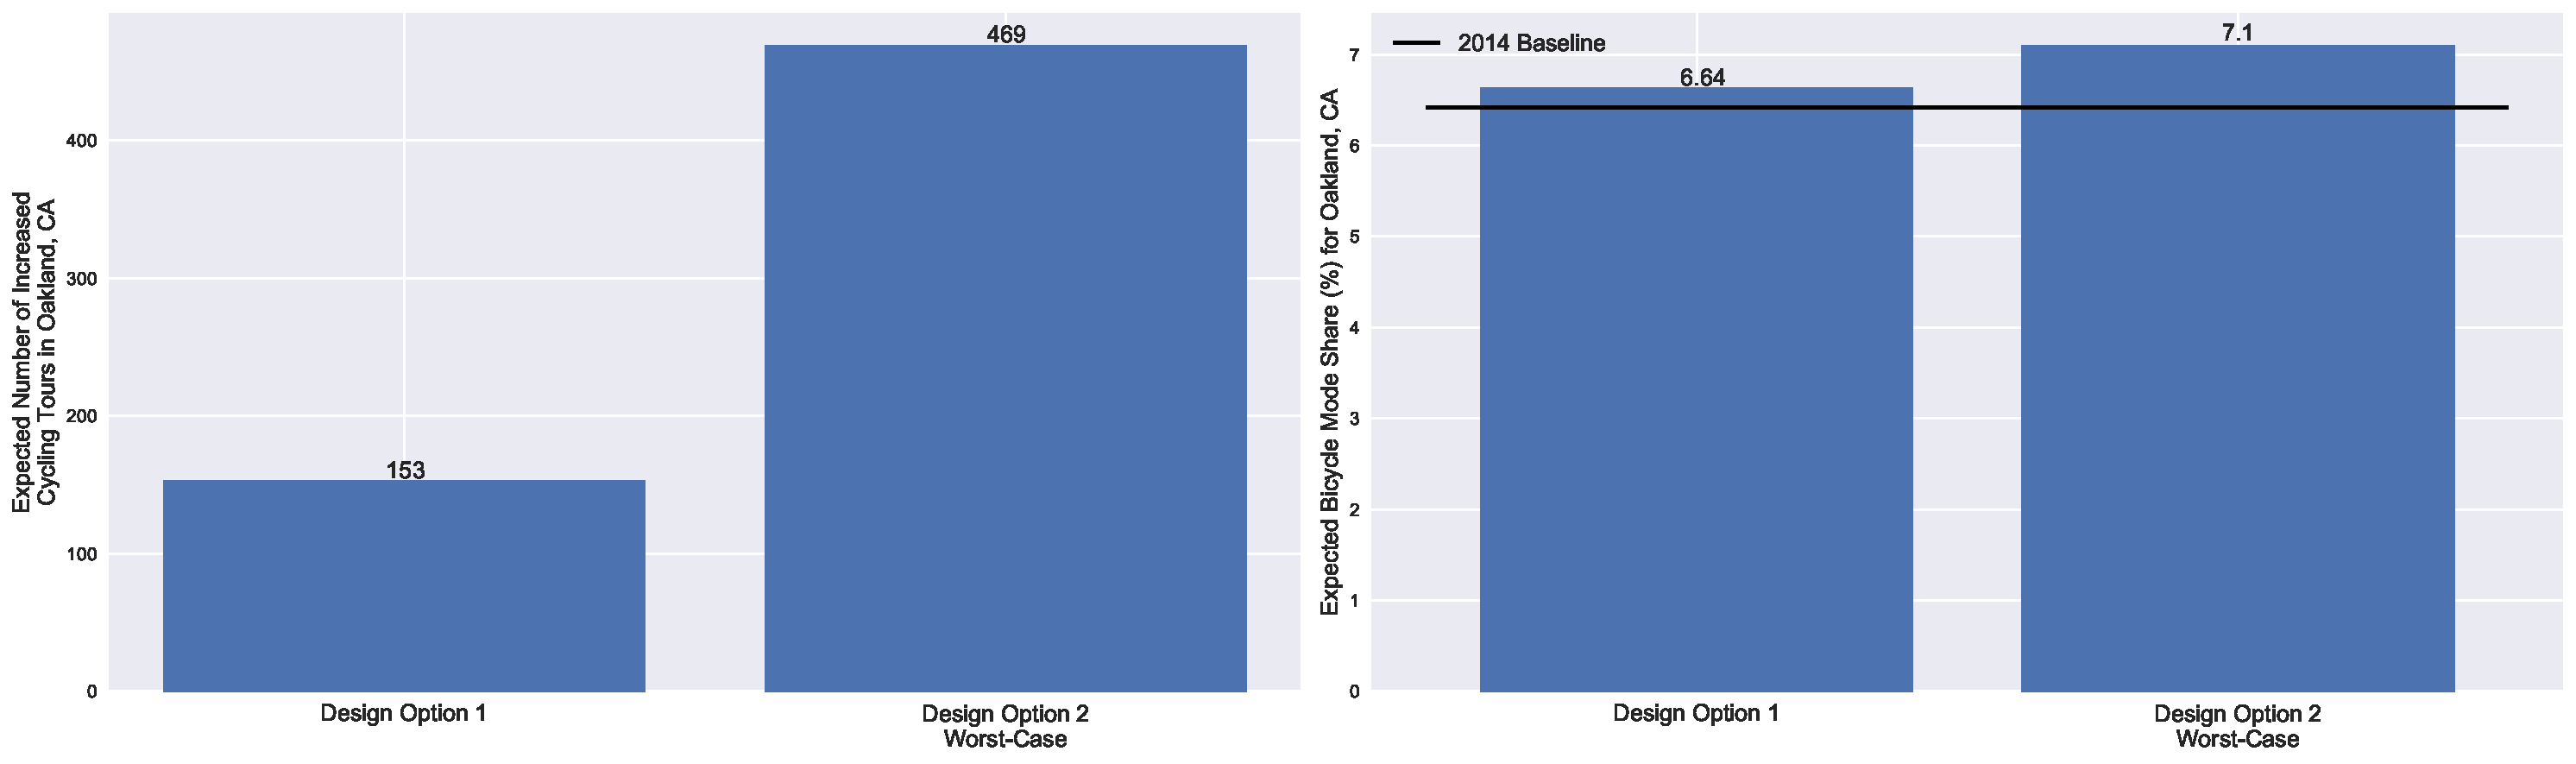
\includegraphics[width=\textwidth]{../images/forecast_results}
    \caption{Forecast results for the hybrid decision tree-logit model}
    \label{fig:forecast_results}
\end{figure}

There are two main findings from this exercise. First, the substantive finding is that keeping the bike lanes on Telegraph Avenue from 46th to 52nd Streets makes a large difference in terms of bicycle demand because that roadway segment is likely to be traversed by many potential cyclists and because sharrows were not associated with a high levels of bicycle usage. Secondly, the methodological finding of this case study is that the combined zone of likely travel and hybrid tree-logit model is sensitive to roadway level variables, as expected. As shown by this case study, the proposed methodology is responsive to changes as small as replacing 6 blocks worth of sharrows with bicycle lanes.

\section{Conclusion}
\label{sec:conclusion}
In this chapter, I introduced a method for incorporating roadway-level variables into discrete choice models. Intuitively, the proposed methodology works as follows. First, for each individual, a geographic buffer is drawn around the shortest path between the individual's origin and destination. The buffer size is chosen so that the buffer contains the roadways that an individual is likely to traverse if the individual were to bicycle. The region denoted by this buffer is referred to as the ``zone of likely travel.'' Next, for all roadways in the zone, the variables of interest are calculated (e.g. does tthis roadway have a bicycle lane, what is the speed limit on this roadway, etc.). These variables are then aggregated to the level of the zone. In this chapter, such aggregation was done by computing deciles of continuous variables and means of continuous and discrete variables. After variable aggregation, each zone of likely travel was ``scored'' by a decision tree. The decision tree was constructed by using whether each individual bicycled as the dependent variable and using the aggregated variables for each zone as explanatory variables. Since each ``score'' is a mapping from a particular output node of the decision tree, membership in each output node was added to the bicycle utility function of a traditional discrete choice model using dummy variables.

Section \ref{sec:zone_of_likely_travel} highlighted the ways that the proposed methodology addresses theoretical shortcomings of previous methods. Empirically, Section \ref{sec:application} showed that the new procedure out-performed traditional discrete choice models that failed to incorporate roadway-level variables and that these performance improvements held both in-sample and out-of-sample and with multiple metrics. Finally, the case study showed that the proposed technique is sensitive to the roadway-level variables and their spatial configuration---sensitive enough to show real differences between two proposed bicycle infrastructure investments in Oakland, California.

All together, this chapter presents a new method for incorporating roadway level variables into discrete choice models. The proposed methodology has expected theoretical benefits over other methods for incorporating roadway-level variables into discrete choice models, and there are empirical benefits to be gained over not incorporating such roadway-level variables. Hopefully, future work will lead to more case studies of the proposed methodology and also to quantitative comparisons with methods based on geographic buffers around points, bicycle-environment factors, and combined route and mode choice models. From a methodological standpoint, it would also be interesting to investigate the extent to which this chapter's proposed methods is able to reduce the spatial dependence of the residuals from one's choice models.

\newpage
\bibliography{ch_2}

\end{document}